\documentclass{article}
\usepackage{graphicx}
\usepackage{amsmath}
\usepackage{pgfplots}
\usepackage{tikz}
\usepackage{txfonts}
\usepackage{physics}
\usepackage{hyperref}
\usepackage[a4paper, top=1cm, bottom=2cm, left=2cm, right=2cm, includehead, includefoot]{geometry}
\pgfplotsset{compat=1.18}

\begin{document}
\noindent
Physics 4A - Classical Mechanics \hfill Prof. Roger King

\noindent\rule{\textwidth}{0.4pt}

\begin{center}
    \textbf{\LARGE Chapter 3 - Vectors} \\
    \vspace{12pt}
    \large Aaron W. Tarajos \\
    \textit{\today}
\end{center}

\noindent\rule{\textwidth}{0.4pt}

\section*{3.1 Vectors and Their Components}
\subsection*{key ideas}
\begin{itemize}
	\item Scalars consist of only magnitude and are subject to the ordinary rules of algebra.
	Vectors consist of magnitude and direction and are subject to the rules of vector algebra.
	\item Two vectors $\va{a}$ and $\va{b}$ can be added geometrically by drawing them at common scales and place them head to tail.
	The vector $\va{s}$ that connects the head and the tail is the summed vector.
	To subtract a vector switch the direction of the one you are subtracting and then proceed as if you were adding them.
	\item The scalar components, $(a_x, a_y, a_z, \dots)$, of a vector $\va{a}$ are found by dropping perpendicular lines from the ends of
	$\va{a}$ onto the coordinate axes. In two dimensions, the components are given by;
	\[
		a_x = a \cos{\theta} \quad \text{and} \quad a_y = a \sin{\theta}
	\]
	and the magnitude and orientation by;
	\[
		a = \sqrt{a_x^2 + a_y^2} \quad \text{and} \quad \tan(\theta) = \frac{a_y}{a_x}
	\]
\end{itemize}

\subsection*{3.1.1 Vectors and Scalars}
\textbf{Motion:}
	A particle moving along a straight line can move in two directions, which can be represented as positive or negative motion.
	For a particle moving in three dimensions, using just a plus or minus sign is insufficient; vectors are needed to represent both direction and magnitude.
\vspace{12pt}\\
\textbf{Vectors:}
    A vector has both magnitude and direction and follows specific rules for combination.
    Vector quantities: These are physical quantities that have both magnitude and direction, such as displacement, velocity, and acceleration.
\vspace{12pt}\\
\textbf{Scalars:}
    Physical quantities that do not have a direction, like temperature, pressure, energy, mass, and time.
    Scalars are handled using regular algebra, and a single value (with a sign) specifies them.
\vspace{12pt}\\
\textbf{Displacement:}
    The simplest vector quantity, which represents a change in position.
    A vector representing displacement is called a displacement vector.
    The arrow from point A to B shows displacement, and vectors with the same magnitude and direction (even if shifted) represent the same displacement.

\subsection*{3.1.2 Adding Vectors Geometrically}
Given a particle that moves from A to B and then B to C.
We represent the overall displacement, regardless of the path taken, as two displacement vectors AB and BC.
The net displacement is the \textbf{vector sum} AC.
\begin{center}
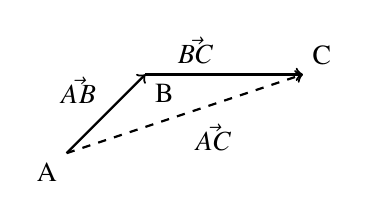
\begin{tikzpicture}[scale=1]
    % Points
    \coordinate (A) at (0,0);
    \coordinate (B) at (1,1);
    \coordinate (C) at (3,1);

    % Vectors
    \draw[thick,->] (A) -- (B) node[midway,above left] {$\vec{AB}$};
    \draw[thick,->] (B) -- (C) node[midway,above left] {$\vec{BC}$};
    \draw[thick,dashed,->] (A) -- (C) node[midway,below right] {$\vec{AC}$};

    % Points Labels
    \node[below left] at (A) {A};
    \node[below right] at (B) {B};
    \node[above right] at (C) {C};
\end{tikzpicture}
\end{center}
The order of the addition does not matter. This is the commutative law;
\[
	\va{a} + \va{b} = \va{b} + \va{a}
\]
While adding two vectors works the way someone may intuitively guess, subtracting is a little different than scalar subtraction.
\[
	\va{d} = \va{a} - \va{b} = \va{a} + (-\va{b})
\]
The vector being subtracted is changed to the opposite direction and then added.

\subsection*{3.1.3 Component Vectors}
\subsubsection*{Vector Components}
A \textit{component} of a vector is the projection of the vector on an axis. To find the projection of a vector along an axis, we draw perpendicular lines from the two ends of the vector to the axis.
The projection of a vector on the $x$ axis is its $x$ component, and similarly the projection on the $y$ axis is the $y$ component.
This process of finding the components of a vector is called \textit{resolving} the vector.
A component of a vector has the same direction (along an axis) as the vector.
If we were to reverse vector $\vec{a}$, then both components would be negative, and their arrowheads would point toward the negative $x$ and $y$ directions.

\subsubsection*{Finding the Components}
We can find the components of $\vec{a}$ geometrically from the right triangle:
\[
a_x = a \cos \theta \quad \text{and} \quad a_y = a \sin \theta
\]
where $\theta$ is the angle that vector $\vec{a}$ makes with the positive $x$ axis, and $a$ is the magnitude of $\vec{a}$.
We arrange those components head to tail, and then complete a right triangle with the vector forming the hypotenuse, from the tail of one component to the head of the other.

\subsubsection*{Component Notation vs Magnitude-Angle Notation}
Once a vector has been resolved into its components along a set of axes, the components themselves can be used in place of the vector.
It can also be given by its components $a_x$ and $a_y$. Both pairs of values contain the same information. If we know a vector in component notation ($a_x$ and $a_y$) and want it in magnitude-angle notation ($a$ and $\theta$), we can use the equations:
\[
a = \sqrt{a_x^2 + a_y^2} \quad \text{and} \quad \tan \theta = \frac{a_y}{a_x}
\]

\subsubsection*{Three-Dimensional Vectors}
In the more general three-dimensional case, we need a magnitude and two angles (say, $a$, $\theta$, and $\phi$) or three components ($a_x$, $a_y$, and $a_z$) to fully specify a vector.

\end{document}
